\documentclass[11pt]{article}

\usepackage[margin=1in]{geometry}
\usepackage[T1]{fontenc}
\usepackage{lmodern}
\usepackage{microtype}
\usepackage{graphicx}
\usepackage{booktabs}
\usepackage{array}
\usepackage{enumitem}
\usepackage{amsmath}
\usepackage{xcolor}
\usepackage{xspace}
\usepackage{hyperref}

\hypersetup{
  colorlinks=true,
  linkcolor=blue!55!black,
  citecolor=blue!55!black,
  urlcolor=blue!55!black,
  pdftitle={RepoPact: Repository-Native Governance for Durable Human-Agent Software Engineering},
  pdfauthor={Jeremy Shows}
}

\newcommand{\repo}{\textsc{RepoPact}\xspace}
\newcommand{\mainbranch}{development \texttt{main}}
\newcommand{\snapshot}{\texttt{6d782116fc9762da00439cf079d0f50585fea52}}

\title{RepoPact: Repository-Native Governance for Durable Human-Agent Software Engineering}
\author{Jeremy Shows\\ForgeWire Labs}
\date{September 14, 2026}

\begin{document}
\maketitle

\begin{abstract}
Agentic software engineering distributes work across humans, coding agents, machines,
model providers, and execution sessions. Source code usually survives these handoffs, but
the governing state around it often does not: intent, authority, invariants, decisions,
acceptance criteria, provenance, and evidence may remain in conversations, local memory,
issue trackers, or one operator's head. We present \repo, a repository-native governance
kernel for durable human-agent software engineering. It stores governing project state as
typed, version-controlled records alongside the artifact being governed, so a fresh human
or agent can recover represented work state, authority boundaries, invariants, decisions,
evidence, provenance, lifecycle, and known violations without predecessor-private context.
We call this property \emph{governance continuity}.

\repo models the repository as six layers: typed records, work-item lifecycle, invariant
monitoring, a typed enforcement lattice, deterministic derived views, and a brownfield
adoption boundary. Its central primitive is the binding invariant, a declared guarantee
coupled to rationale, escalation, and, where logically possible, machine enforcement.
The implementation has evolved from a Python reference system into a canonical Rust
semantic engine with compatibility tooling and a Tauri 2 Workbench. RepoPact 3.1.0 is the
stable public boundary and ships the canonical engine, local-first verification/release
surface, additive graph capability, and optional assurance-mapping capability in the
Python/Rust package. WI063's graph implementation is substantially operational but remains
active at 37/40 satisfied criteria; WI065's app-private mobile acquisition checkpoint is
real but active at 4/9 satisfied criteria. Windows, Linux, and Android evidence exists,
while macOS and iOS still require platform-specific validation. RealRunner has crossed the
real-model-exercised boundary, but comparative cross-model results remain pending.
\end{abstract}

\paragraph{Keywords:} agentic software engineering; human-agent collaboration; repository
governance; governance continuity; software invariants; durable project state;
evidence-gated workflows; brownfield adoption; provenance typing; conformance.

\section{Introduction}

A coding agent is given a task, loads context, changes code, and finishes a session. The
next session may use another model, machine, developer, or client. The source tree
survives, but the reason the change was safe may not. The missing state includes what the
work was trying to accomplish, what was authorized, what must not be weakened, which
decisions were already made, what counts as completion, what evidence exists, what remains
uncertain, and what should happen next.

These facts are commonly scattered across chat logs, prompt transcripts, local scratchpads,
issue trackers, private planning documents, model memory, and operator knowledge. We
originally described the symptom as session amnesia. The deeper problem is governance
discontinuity: a project may preserve its files while losing the durable state that tells
the next worker how those files may legitimately change.

The repository is the one artifact every legitimate participant already needs to obtain. It
is persistent, diffable, reviewable, replicated, branchable, and tied to source, tests,
history, and change-control mechanisms. \repo makes that same repository carry the durable
state required to govern the work. A fresh human or agent should be able to clone the
repository and recover not only the code, but the represented governed state needed to
continue responsibly.

Repository instruction files such as \texttt{AGENTS.md}, architecture decision records,
issue trackers, policy-as-code systems, and runtime sandboxes each cover part of this
problem. \repo does not replace them. It provides a durable governance layer in which
intent, authority, evidence, lifecycle, provenance, conformance, and drift can meet.
\texttt{AGENTS.md} and similar instruction files tell an agent how it should behave.
\repo records durable project state around that behavior and validates, and where
enforceable can enforce, whether the repository still respects its declared contract.

\begin{figure}[t]
  \centering
  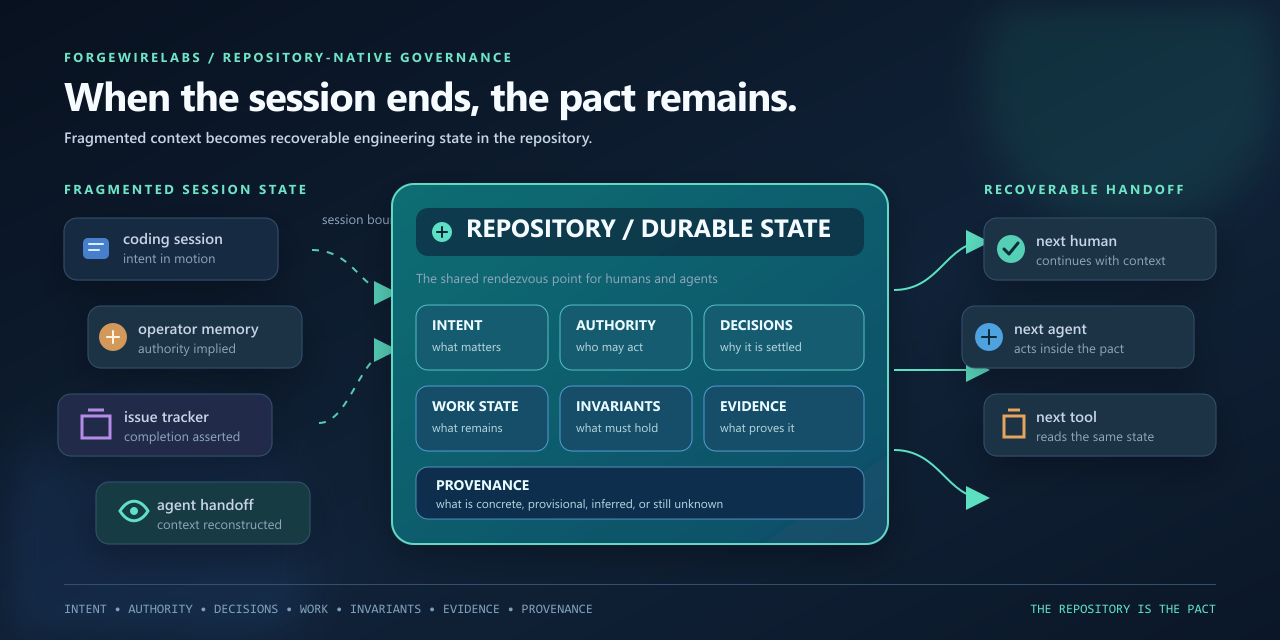
\includegraphics[width=\linewidth]{figures/repopact-hero-social.png}
  \caption{\repo's product model: fragmented session state is converted into durable,
  inspectable repository state that supports a recoverable handoff to the next human,
  agent, or tool. The illustration is a product diagram, not a benchmark result.}
  \label{fig:hero}
\end{figure}

This paper makes six contributions:
\begin{enumerate}[leftmargin=*]
  \item a repository-native governance model organized as a six-layer kernel;
  \item governance continuity, defined as recoverability of represented governed state
        across worker and session transitions;
  \item the binding invariant as a first-class primitive coupled to rationale,
        escalation, and possible enforcement;
  \item a typed enforcement lattice whose invariant kinds predict the required enforcer;
  \item a concrete-record brownfield trilemma and provenance-typed resolution for
        epistemically uncertain reconstruction; and
  \item a falsification-oriented evaluation program based on the packaged implementation,
        conformance suite, findings, naturalistic cases, and pre-registered benchmarks.
\end{enumerate}

\section{Model}

\subsection{Six layers of the governance kernel}

The kernel is deliberately repository-native rather than runtime-native. L0 is a typed
record store for work, decisions, invariants, evidence, ownership, and provenance. L1
adds work-item lifecycle automata and explicit authority states. L2 is an invariant monitor
that checks structural, semantic, and cross-record conformance. L3 is a typed enforcement
lattice. L4 produces deterministic derived views such as dashboards and graph projections.
L5 is the brownfield adoption boundary where external plans and uncertain reconstruction
enter the governed tree.

The layers constrain one another without pretending they solve the same problem. A
dashboard is derived and therefore generated, not a second hand-maintained ledger. An
invariant may be binding even when its current enforcer is human review. An adopted claim
may be useful while still carrying \texttt{inferred} or \texttt{provisional} provenance.

\subsection{Governance continuity}

Let $s$ be a repository state, $G(s)$ its represented governance projection, and
$V(s)$ its known violations. A worker transition $h$ is governance-continuous for
represented state when a fresh legitimate worker can obtain a clean clone and recover
\[
  \operatorname{recover}_h(\operatorname{clean\_clone}(s)) = \langle G(s), V(s)\rangle
\]
without predecessor-private context. This is a recoverability claim, not an omniscience
claim. Facts that never entered the repository remain outside the model. A nonconformant
repository can still be governance-continuous if the next worker faithfully recovers its
records and the violations that make it nonconformant.

The practical falsification target is any load-bearing state required to continue
legitimate work that exists only in a specific worker, machine, provider, UI cache, or
conversation while the system claims the repository is authoritative for that state.

\subsection{Authority and provenance}

The lifecycle state \texttt{proposed} is a durable candidate state, not an accidental
synonym for \texttt{active}. It captures work that deserves visibility but has not yet
received implementation authority. Provenance types distinguish \texttt{concrete},
\texttt{provisional}, and \texttt{inferred} claims. This resolves a brownfield
trilemma: a concrete-only migration cannot always be total, faithful, and closed at once
when the source material is incomplete or contradictory.

Provenance does not make a cyclic dependency graph acyclic, turn an unsupported relation
into a valid one, or make uncertain completion evidence sufficient. Structural residue is
reported explicitly. The point is to give a worker an honest third option between
fabrication and deletion.

\subsection{Typed enforcement lattice}

RepoPact distinguishes state, state-fixpoint, transition, temporal, relational, and meta
invariants. A state invariant can often be decided from one tree. A state-fixpoint
invariant needs a generator and validator, such as dashboard equality. A transition
invariant needs a base and head, such as acknowledgement for a frozen-surface change. A
temporal invariant needs history or review. A relational invariant needs contracts and
refinement semantics. A meta invariant often remains partly dependent on human judgment.
The distinction prevents a validator from being presented as a universal runtime guard.

\section{Reference implementation}

The current implementation has one semantic authority. A canonical Rust engine provides
repository discovery and modeling, schema-backed validation, structured diagnostics,
dashboard rendering, relationship graphs, deterministic analysis, typed work-item creation
and editing for proven fields, lifecycle transition, and content-addressed mutation
planning and recovery. Python compatibility tooling speaks a versioned local process
protocol to that engine. Native clients such as the Tauri Workbench call the same Rust
crates directly.

\begin{sloppypar}
The stable public CLI retains \texttt{init}, \texttt{adopt}, \texttt{import-plan},
\texttt{new}, \texttt{validate}, \texttt{dashboard}, \texttt{spec},
\texttt{check-frozen}, and \texttt{doctor}, and adds \texttt{verify}, \texttt{release},
\texttt{graph}, \texttt{assurance}, and bounded \texttt{admission} and
\texttt{approval} operations. These additions identify the 3.1.0 package boundary.

The package does not imply that external platform or research gates are closed.
\end{sloppypar}

\subsection{Workbench and platform posture}

The Workbench is a Tauri 2 client of the canonical engine, not a second source of truth.
It presents repository state, validation, work lifecycle, decisions, evidence,
relationships, analysis, session state, and governed mutations through user-facing views.
The release standard is operator control parity for core governance, not pixel-perfect
identity with the CLI.

Windows, Linux, and Android bring-up evidence exists. Android evidence includes a real SAF
acquisition checkpoint proving directory and archive import, app-private staging, registry
persistence, picker cancellation, and permission/log-privacy checks on an emulator. The
mobile repository architecture treats app-private workspaces as ordinary repositories and
SAF/archive mechanisms as acquisition transports; explicit export/share-back and the
Workbench mutation cycle remain open in WI065. macOS and iOS remain intended targets and
require native platform-specific validation. A current Windows snapshot is shown in
Figure~\ref{fig:workbench}; it is an implementation capture, not evidence that every
Workbench or mobile criterion is complete.

\begin{figure}[t]
  \centering
  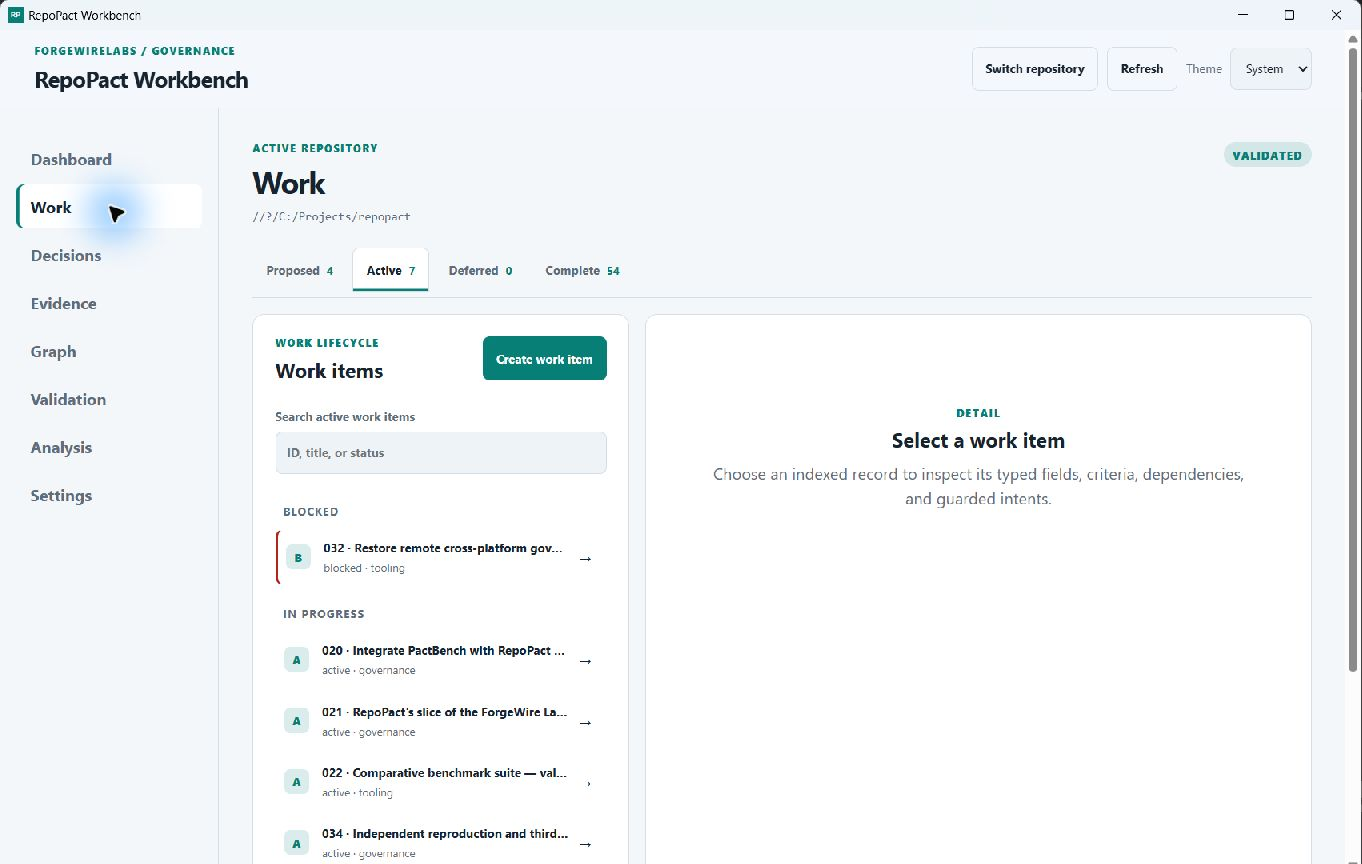
\includegraphics[width=0.96\linewidth]{figures/workbench-governance.jpg}
  \caption{RepoPact Workbench on Windows showing a validated repository and the governed
  work-item surface at the 3.1.0 release-candidate snapshot. This is an implementation
  capture, not evidence that every Workbench capability or platform gate is complete.}
  \label{fig:workbench}
\end{figure}

\subsection{Local-first verification and release boundary}

WI046 established the local-first verification and release architecture. Local validation,
evidence, release inspection, and build checks are shipped 3.1.0 package surfaces rather
than future work. That architecture still does not make all external admission gates green.
In particular, local verification success is not remote enforcement closure, and protected
admission remains incomplete.

\section{Evaluation program}

\subsection{Pre-registered comparative studies}

The comparative program holds source, task, model, and harness constant while varying the
registered governance or context condition. S1--S8 cover guarantee-violation detection,
cross-session recovery, multi-agent coordination, context-token economy, drift detection,
defensive security, enforcement closure, and governance continuity with clean-clone
orientation cost. S8 was registered before graph-enabled runs.

The program is pre-registered and partially implemented. Deterministic task materialization,
the driver, scoring, drift/security instrumentation, and harness infrastructure exist. WI022
AC-5 has crossed the real-model-exercised boundary through a reportable three-task RealRunner
smoke with reconciled telemetry and deterministic grading. That smoke validates runtime and
evidence plumbing, not comparative performance; WI022 AC-3 remains pending because the
two-model-family comparative program has not been completed. S8's secondary cost metrics
include time, tokens, tool calls, file reads, bytes read, and repository-wide search
operations.

\subsection{PactBench}

PactBench measures whether agents silently weaken declared guarantees less often when
governed context is present. A task creates pressure to take a shortcut that would violate
a declared guarantee. Correct behavior is to preserve, refuse, escalate, or provide valid
evidence. The scorer records silent weakening, preservation, escalation, and false
stopping. The suite includes correctness and security classes, evidence-fabrication
pressure, context-injection cases, real fixtures, a model-agnostic harness, deterministic
self-tests, subprocess support, and drift experiments.

\section{Results and findings}

The reflexive findings register contains nineteen entries. ``Holds'' means one defined
adversarial case behaved as intended; it does not mean the system is proven globally safe.
Table~\ref{tab:findings} summarizes the current register.

\begin{table}[t]
\centering
\small
\begin{tabular}{p{0.10\linewidth}p{0.11\linewidth}p{0.16\linewidth}p{0.52\linewidth}}
\toprule
ID & Hypothesis & Severity & Finding and current disposition \\
\midrule
F-001 & H2 & major & \texttt{spec} crashed on an init-fresh repository; fixed and re-verified. \\
F-002 & H4 & minor & Frozen-surface checks missed working-tree edits; fixed and re-verified. \\
F-003--F-007 & H1--H7 & holds/major & Evidence gating, lifecycle, frozen-surface, and brownfield cases held or were repaired. \\
F-008 & H7 & major & An adopter ignore rule swallowed evidence; warning and repair guidance added. \\
F-009--F-014 & H6--H7 & holds/major & Clean-room adoption, import-plan, doctor, lifecycle, and authority-state cases held or shipped. \\
F-015 & H7 & major & Linked-worktree validation produced false errors; fixed in 3.0.2 and re-verified. \\
F-016 & H6,H12 & minor & README and canonical JSON identity drifted; open reconciliation item. \\
F-017 & H12 & minor & Doctor documentation used a stale source-of-truth path; fixed and re-verified. \\
F-018 & H6,H7 & major & Evidence chronology depended on wall-clock timestamps; deterministic Git-recording basis added. \\
F-019 & H14 & major & Preflight/post-change validation did not prevent an autonomous worker's first write before admission; protected-admission guard and cross-platform proof pending. \\
\bottomrule
\end{tabular}
\caption{Current findings through the 3.1.0 release-candidate snapshot. The grouped rows
preserve the complete register while keeping the submission table legible.}
\label{tab:findings}
\end{table}

The findings changed the design rather than being edited out of the story. F-001 closed a
surface gap. F-002 exposed the practical boundary of local protected-surface checks. F-008
showed that an ignored evidence directory can make a repository validate on one disk while
a clean clone loses proof. F-010 motivated \texttt{import-plan}; F-011 motivated
\texttt{doctor}; and F-014 established that a missing authority state can be repaired while
the resolution trace remains recoverable.

F-015 corrected physical checkout-topology handling. F-016 remains an open identity drift
item: canonical metadata is authoritative, and documentation must not silently redefine it.
F-017 corrected a repair-path source-of-truth reference. F-018 replaced drifting wall-clock
chronology with a deterministic Git-recording basis.

F-019 is the important negative result for enforcement claims. RepoPact could durably
require preflight and detect an invalid sequence after the fact while still lacking a
mechanism that prevented an autonomous worker's first write before admission. This narrows
the claim: repository governance and post-change verification are not equivalent to
pre-execution containment. Protected admission requires a distinct runtime or OS-backed
enforcement boundary. The architecture is accepted in WI050 and decision 0038, but the
executable guard and cross-platform proof remain pending.

\section{Repository Orientation Graph}

Governance continuity says the state is recoverable; it does not say a fresh worker can
recover it cheaply. S8 therefore measures orientation cost separately from correctness.
The current 3.1.0 implementation provides a substantially operational, active, derived,
versioned Repository Orientation Graph substrate with deterministic rebuild, incremental/full
convergence, language-aware semantic extraction, working-tree overlays, explicit freshness
and coverage state, metadata/topology adapters, bounded public query/orientation operations,
and Workbench repository-map behavior. WI063 has 37/40 criteria satisfied; its remaining
criteria cover cross-platform usability/normalization, the preregistered S8 R1 evaluation,
and the final closeout inventory/gate.

The graph remains non-authoritative: source and governance records remain the source of
truth, and graph output does not authorize mutation. Any graph-enabled condition must be
added through a dated amendment and measured against the pre-registered no-graph baseline.
The implementation evidence supports operational maturity, not a causal claim that ROG
improves orientation or complete repository understanding.

\subsection{Assurance and control mapping}

WI051 is completed with an optional, provider-neutral assurance/control mapping model. A
mapping distinguishes framework mapping, applicability conclusion, implemented control,
operating evidence, and independent audit or certification, while resolving implementation
and evidence references, reviewer rationale, stale framework/review and reference drift,
sensitive-evidence boundaries, and documentation claim basis. ForgeWire is an adopter
example rather than a hard-coded framework. RepoPact governs assurance mappings and evidence
boundaries; it does not infer legal compliance, certification, SOC~2, HIPAA, PCI, GDPR, or
any other external conclusion from a stored mapping.

\section{Threats to validity}

RepoPact was distilled from the author's own agentic engineering practices, so the
progenitor repository is confirmatory rather than independent. Much evidence comes from
one primary operator working with several AI systems. Current evidence is not
representative of every enterprise, regulated environment, monorepo, or many-agent team.
One adversarial case is not universal safety; benchmark curation and baseline fairness can
overstate value; token and cost measurements depend on provider and retrieval behavior; and
synthetic drift/security tasks may not reflect production conditions.

The implementation currently defines much of the operational semantics, although the
conformance suite provides an observable target for alternate implementations. Provenance
can be misused if users treat inferred or provisional records as proof. A polished
Workbench can create a false impression of operator parity, so UI claims must distinguish
implemented, wired, validated, and planned controls. Finally, the active graph could be
designed around future evaluation tasks; preregistered S8 measures and amendment rules
mitigate that risk.

\section{Conclusion and future work}

Agentic software engineering has a continuity problem in addition to a context problem.
Code can survive a session while the governing state around that code disappears. \repo
addresses this by making the version-controlled repository carry a typed governance layer.
A fresh human or agent can recover represented intent, authority, evidence, decisions,
provenance, invariants, known violations, and next work without starting over.

The evaluation remains intentionally incomplete. Real failures changed the design. Real
cases held. RealRunner has crossed the real-model-exercised boundary, but the smoke validates
runtime and telemetry plumbing rather than comparative performance. The enforcement-closure
observation motivated a hypothesis rather than being treated as proof. Governance continuity
and graph-enabled orientation remain registered prospective work, not empirical improvement
results.

Future work includes the WI022 two-model-family comparative program; enforcement-closure and
S8 studies outside ForgeWire-controlled repositories; third-party reproduction; completion
of WI063's cross-platform usability, R1 execution, and closeout inventory; completion of
WI065's Workbench mutation, explicit export/share-back, and end-to-end mobile runtime
acceptance; native macOS and iOS validation; provenance-preserving external ingestion;
stronger temporal and relational invariants; and independent conformance implementations.

\section*{Reproducibility and artifact availability}

This submission is frozen against the RepoPact 3.1.0 release-candidate snapshot:
\begin{quote}\texttt{\scriptsize\snapshot}\end{quote}
The stable software boundary is 3.1.0. The snapshot identifies the implementation and
evidence state used for this paper; active WI063/WI065 work is labelled as incomplete even
where code and concrete checkpoints exist. The repository contains the formal model,
benchmark protocol, threats and findings registers, conformance suite, evidence records,
Workbench source, and launch-readiness records. The arXiv package is a clean source package
under \texttt{research/arxiv}; its
figures are copied into the package so compilation does not depend on absolute workstation
paths. Comparative model results are not included in this version.

The package was intended for a clean LaTeX build from its own directory. No arXiv account,
license selection, endorsement, or submission was performed as part of this preparation.

\nocite{agentsmd,memgpt,nygard,opa,conftest,evolutionary,backstage,swebench,sweevo}
\bibliographystyle{plain}
\bibliography{references}

\end{document}
